%In the fast-evolving landscape of healthcare, seamless collaboration between multiple organizations is essential to ensure the highest standard of patient care. We delve into the application of Trusted Execution Environment (TEE) to facilitate the secure exchange of event logs between three pivotal actors: an esteemed hospital, a specialized clinic, and a leading pharmaceutical company. This innovative approach fosters a robust and trustworthy ecosystem where sensitive patient data can be shared securely, promoting seamless collaboration for the betterment of patient outcomes.

%Sintetizza il processo tra ospedale azienda farmaceutica e struttura specializzata
\begin{figure}[t]
\centering
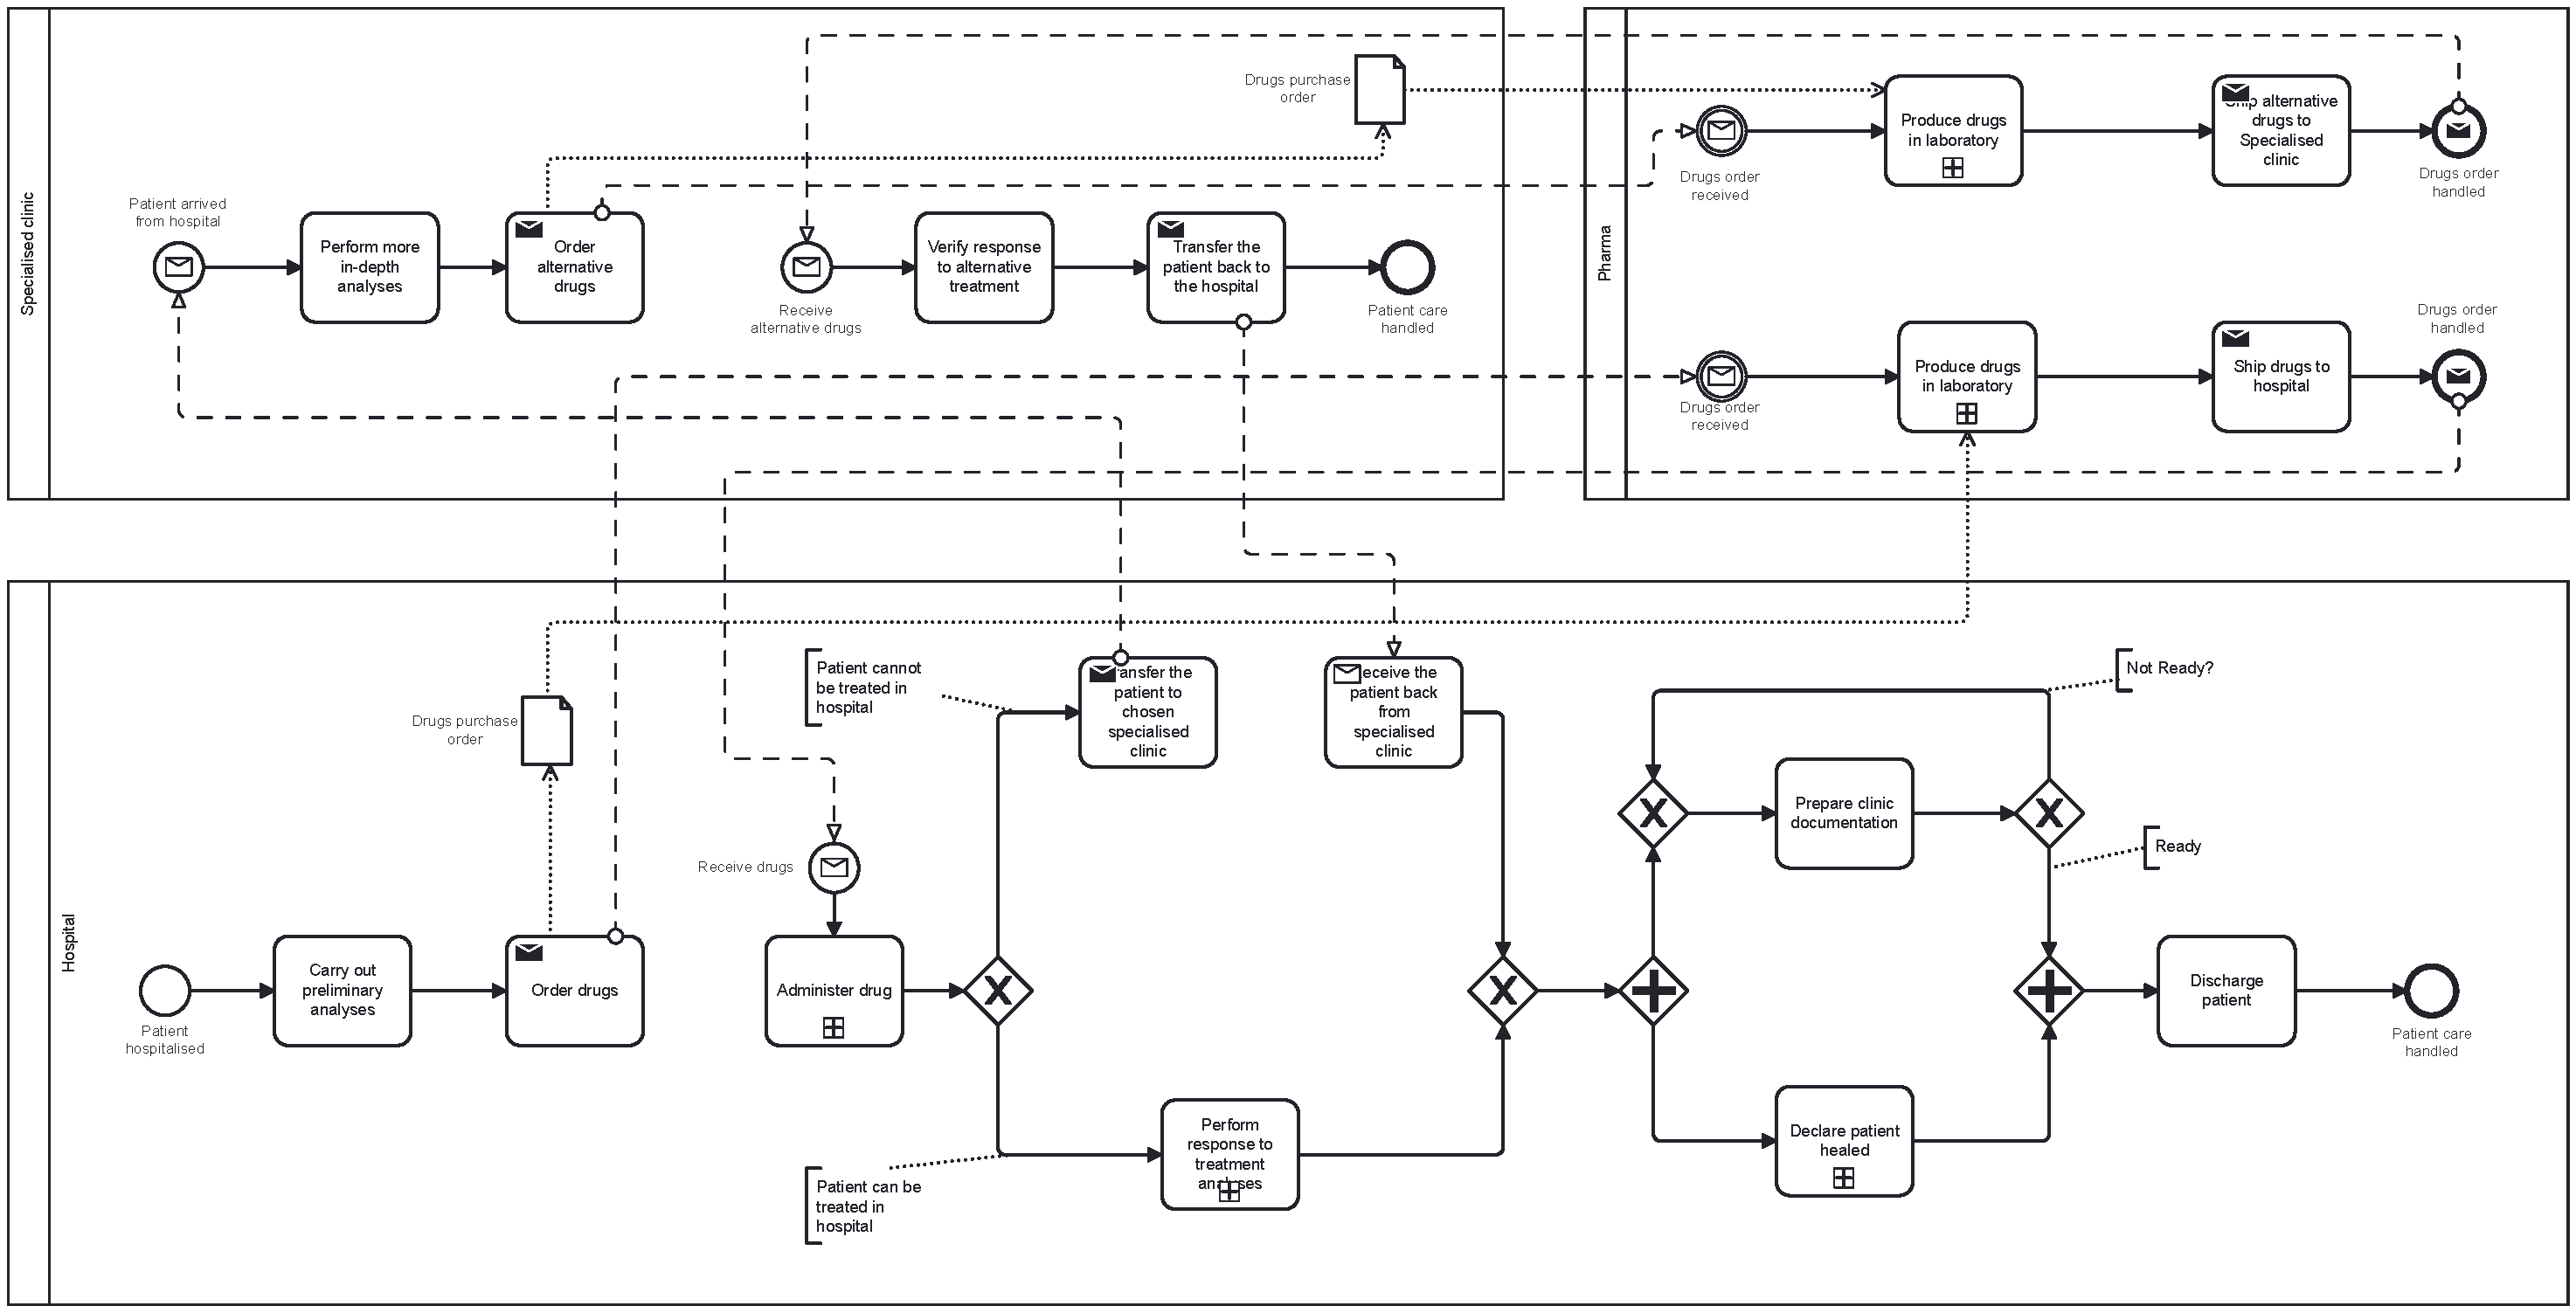
\includegraphics[width=10 cm]{content/figures/healthcare_scenario.pdf}
\caption{BPMN Healthcare Scenario}
\label{fig:BPMN_Healthcare}
\end{figure}
\section{Motivating Scenario}\label{sec:motivating}
\todo[inline]{It can be reduced}
In the medical field, cooperation between different structures is crucial and as illustrated in \cref{fig:BPMN_Healthcare}, many processes are outsourced. 
When a patient enters the hospital, preliminary examinations are carried out and then the hospital company orders the drugs needed to treat the patient from the pharmaceutical company. The pharmaceutical company receives the order and prepares it in the laboratory if the drugs are unavailable, otherwise sends it to the requesting hospital. The hospital will manage the drugs received and check whether the patient can be treated in the hospital or not. If patients require special care, they are transferred to a specialized clinic where more in-depth checks will be carried out. If necessary, the specialized clinic will order drugs from the pharmaceutical company, which will supply them, depending on availability. Once the response to the alternative treatment has been verified, the patient is transferred to the hospital to prepare the dehospitalization. Before discharging the patient, the hospital prepares the necessary clinical documentation. In addition, the hospital also carries out analysis checks and then declares the patient cured to be discharged.
%Storiella sullo scambio e utilizzo dei dati

Any organization that is part of the collaboration environment can make the request to perform process mining operations. For instance, the hospital cooperates with the specialized clinic and the pharmaceutical company, it can decide at any time to analyze the entire process by considering data from all three partners to provide an overview. The hospital requests the necessary data from all companies participating in the cooperation. All companies will send their process data in event log form. In order to mine all data together, the hospital must merge the event logs received. Once the event log has been merged, the hospital can proceed with the execution of the mining algorithm to analyze the entire process.

